\documentclass[a4paper, french]{article}
\usepackage{config}
\author{Vincent Commin \& Louis Leenart}
\date{\today}
\setcounter{secnumdepth}{6}
\begin{document}

\begin{titlepage}
    \begin{flushleft}
        \includegraphics[width=5cm]{UL.jpg}\par
        \centering

        \vspace{13\baselineskip}
        \HRule \\[0.4cm]

        {\Huge
        GIF-4104 - TP 5\par}
        \vspace{0.4cm}
        \HRule
        \vfill
        Équipe 1 : Vincent Commin \& Louis Leenart\medskip \par
    \end{flushleft}
\end{titlepage}

\newpage
\section{Introduction}

Pour ce dernier TP, nous avons eu à implémenter l'algorithme de \href{https://en.wikipedia.org/wiki/PageRank}{\textit{\underline{PageRank}}} en utilisant le moteur \href{https://spark.apache.org/}{\textit{\underline{Apache Spark}}}. L'algorithme consiste à associer un rang à chaque élément d'un graphe orienté. Dans notre cas, les noeuds du graphe représentent des URL, et les arêtes sont les références vers d'autres pages. Concernant l'implémentation, Spark support de nombreux langages et nous avons choisi Java pour sa simplicité d'utilisation ainsi que notre maîtrise du langage.

\section{Notre approche}

Pour implémenter cet algorithme, nous avons suivi la procédure suivante:

\begin{lstlisting}[style=txt]
LECTURE fichier
CONSTRUCTION rdd A PARTIR de fichier

POUR iteration ALLANT DE 0 A 100 FAIRE
    CALCUL rang
FIN POUR

COLLECTE donnees

AFFICHE lien ET rang
\end{lstlisting}

Plus précisément, le calcul du rang pour chacun des liens se faire de la manière suivante:

\begin{lstlisting}[style=txt]
// un élément = id du lien, liste des id de lien qu'il référence
liens : LISTE COUPLE (id, LISTE id)
rangs : LISTE COUPLE (id, rang)
damping_factor : ENTIER

contributions : LISTE COUPLE (id, contribution)
contributions = join(liens, ranks).map(s -> {
    s.gauche.map(n -> {
        n, s.droit / len(s.gauche)
    })
})
rangs = contributions.reduce(+).map(s -> {
    s * damping_factor + 0.15
})
\end{lstlisting}

Après un nombre significatif d'intéractions, le contenu de `rangs` contient les couples `lien : rang`, en sachant que plus le rang tends vers 0, moins il est considéré comme intéressant, et plus il est élevé, plus il est considéré comme pertinent.

\section{Machine utilisée pour les tests de performance}

\begin{center}
    \begin{tabularx}{0.6\textwidth}{|>{\raggedleft\arraybackslash}X|>{\raggedright\arraybackslash}X|}
        \hline
        Modèle & intel i7-8550U \\
        \hline
        Architecture & x86\_64 \\
        \hline
        OS & Archlinux \\
        \hline
        Fréquence CPU & 3.4GHz \\
        \hline
        C\oe urs (physique / logique) & 4 / 8 \\
        \hline
        Ram & 16 Go, 2400 $MT/s$ \\
        \hline
        Java & OpenJDK 11.0.15 \\
        \hline
        Spark Java & 3.2.0 \\
        \hline
    \end{tabularx}
\end{center}

\section{Résultats obtenus}

\begin{center}
    \begin{tabularx}{\textwidth}{c c}
        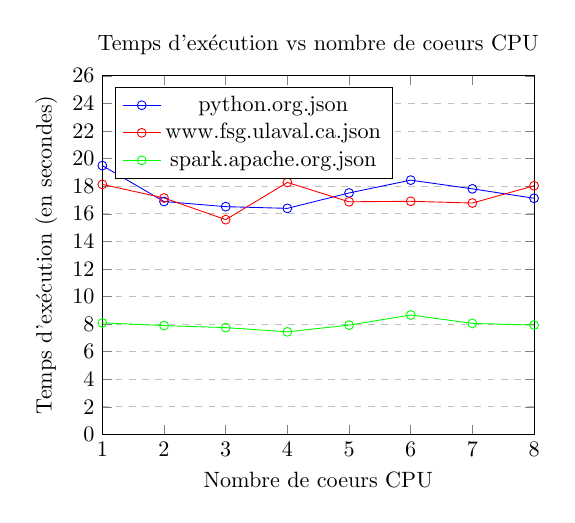
\begin{tikzpicture}[scale=0.8, transform shape]
            \begin{axis}[
                title={Temps d'exécution vs nombre de coeurs CPU},
                xlabel={Nombre de coeurs CPU},
                ylabel={Temps d'exécution (en secondes)},
                xmin=1, xmax=8,
                ymin=0, ymax=26,
                xtick={1,2,3,4,5,6,7,8},
                ytick={0, 2, 4, 6, 8, 10, 12, 14, 16, 18, 20, 22, 24, 26},
                legend pos=north west,
                ymajorgrids=true,
                grid style=dashed,
                ]
                \addplot[color=blue, mark=o] coordinates {(1, 19.491886242)(2,16.889216088)(3,16.516348333)(4,16.392411605)(5,17.508512459)(6,18.437910422)(7,17.808056914)(8,17.124364136)};
                \addplot[color=red, mark=o] coordinates {(1, 18.129680673)(2,17.144475737)(3,15.574049389)(4,18.270912726)(5,16.869163813)(6,16.905354583)(7,16.778233297)(8,18.030930115)};
                \addplot[color=green, mark=o] coordinates {(1, 8.090807218)(2,7.893523972)(3,7.746272639)(4,7.442461376)(5,7.926939141)(6,8.663375522)(7,8.052595936)(8,7.932390062)};
                \legend{python.org.json, www.fsg.ulaval.ca.json,  spark.apache.org.json}
            \end{axis}
        \end{tikzpicture}
        &
        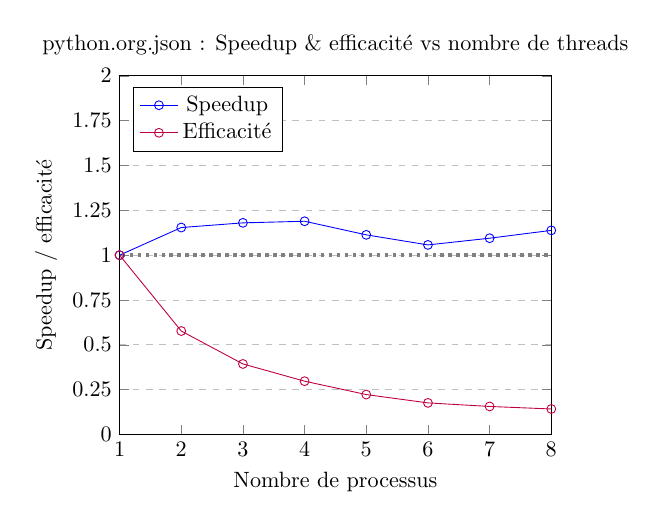
\begin{tikzpicture}[scale=0.8, transform shape]
            \begin{axis}[
                title={python.org.json : Speedup \& efficacité vs nombre de threads},
                xlabel={Nombre de processus},
                ylabel={Speedup / efficacité},
                xmin=1, xmax=8,
                ymin=0, ymax=2,
                xtick={1, 2, 3, 4, 5, 6, 7, 8},
                ytick={0, 0.25, 0.5, 0.75, 1, 1.25, 1.5, 1.75, 2},
                legend pos=north west,
                ymajorgrids=true,
                grid style=dashed,
                ]
                \addplot[color=blue, mark=o] coordinates {(1, 1)(2, 1.154102484)(3,1.18015713)(4, 1.189079844)(5, 1.113280542)(6, 1.057163518)(7, 1.094554355)(8, 1.1382546)};
                \addplot[color=purple, mark=o] coordinates {(1, 1)(2, 0.5770512421)(3,0.3933857099)(4, 0.2972699611)(5, 0.2226561084)(6, 0.1761939196)(7, 0.1563649078)(8, 0.1422818249)};
                \addplot[color=gray, dotted, ultra thick] coordinates {(0, 1)(8, 1)};
                \legend{Speedup, Efficacité}
            \end{axis}
        \end{tikzpicture}
        \\
        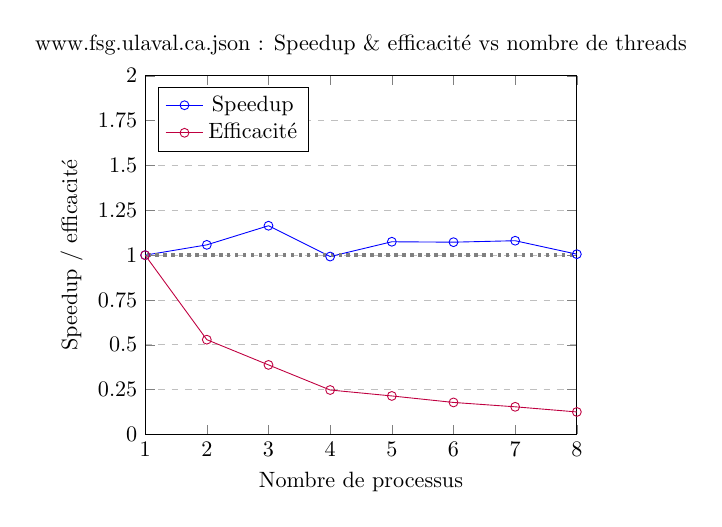
\begin{tikzpicture}[scale=0.8, transform shape]
            \begin{axis}[
                title={www.fsg.ulaval.ca.json : Speedup \& efficacité vs nombre de threads},
                xlabel={Nombre de processus},
                ylabel={Speedup / efficacité},
                xmin=1, xmax=8,
                ymin=0, ymax=2,
                xtick={1, 2, 3, 4, 5, 6, 7, 8},
                ytick={0, 0.25, 0.5, 0.75, 1, 1.25, 1.5, 1.75, 2},
                legend pos=north west,
                ymajorgrids=true,
                grid style=dashed,
                ]
                \addplot[color=blue, mark=o] coordinates {(1, 1)(2, 1.057464862)(3, 1.164095491)(4, 0.9922701151)(5, 1.074723138)(6, 1.072422385)(7, 1.080547657)(8, 1.005476731)};
                \addplot[color=purple, mark=o] coordinates {(1, 1)(2, 0.5287324311)(3, 0.3880318304)(4, 0.2480675288)(5, 0.2149446277)(6, 0.1787370641)(7, 0.154363951)(8, 0.1256845914)};
                \addplot[color=gray, dotted, ultra thick] coordinates {(0, 1)(8, 1)};
                \legend{Speedup, Efficacité}
            \end{axis}
        \end{tikzpicture}
        &
        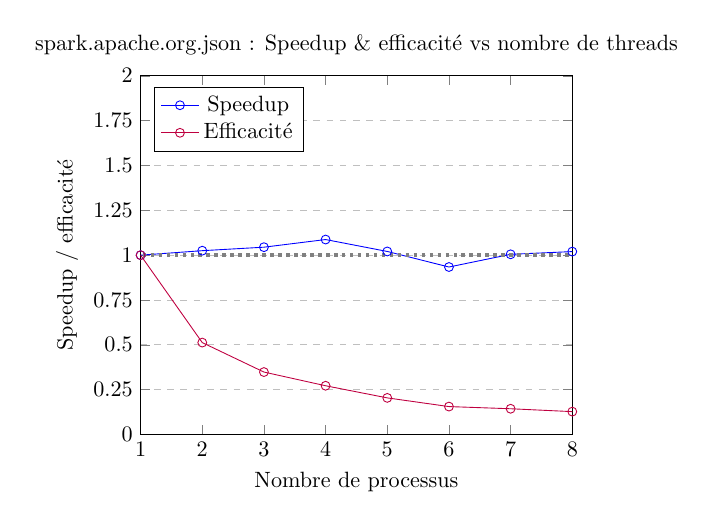
\begin{tikzpicture}[scale=0.8, transform shape]
            \begin{axis}[
                title={spark.apache.org.json : Speedup \& efficacité vs nombre de threads},
                xlabel={Nombre de processus},
                ylabel={Speedup / efficacité},
                xmin=1, xmax=8,
                ymin=0, ymax=2,
                xtick={1, 2, 3, 4, 5, 6, 7, 8},
                ytick={0, 0.25, 0.5, 0.75, 1, 1.25, 1.5, 1.75, 2},
                legend pos=north west,
                ymajorgrids=true,
                grid style=dashed,
                ]
                \addplot[color=blue, mark=o] coordinates {(1, 1)(2, 1.024993051)(3, 1.044477466)(4, 1.087114438)(5, 1.020672302)(6, 0.9339093287)(7, 1.004745213)(8, 1.019970924)};
                \addplot[color=purple, mark=o] coordinates {(1, 1)(2, 0.5124965254)(3, 0.3481591554)(4, 0.2717786096)(5, 0.2041344603)(6, 0.1556515548)(7, 0.1435350304)(8, 0.1274963655)};
                \addplot[color=gray, dotted, ultra thick] coordinates {(0, 1)(8, 1)};
                \legend{Speedup, Efficacité}
            \end{axis}
        \end{tikzpicture}
    \end{tabularx}
\end{center}

\section{Analyse}

Pour mesurer les performances de notre algorithme et sa scalabilité avec le nombre de processus associés, nous avons utilisés les fichiers fournis, présents dans l'archive. Nous avons rencontré de nombreuses difficultés à paramétrer Spark, aussi bien pour le faire fonctionner de façon consistante, que pour spécifier le nombre exacte de CPU disponibles. Malgré tout, nous avons remarqué que Spark utilise plus de ressources qu'imposé. À noter aussi que Spark utilise plusieurs processus pour fonctionner, pour l'ordonnancement des processus et la gestion des ressources, utilisant alors du temps CPU difficile à mesurer.

D'après les graphiques ci-dessus, nous pouvons noter que le temps de calcul décroît légèrement avec l'ajout de cours CPU, cependant la diminution n'est pas significative, et parfois inexistante pour certains fichiers traités. Notamment pour le fichier "python.org.json", le speedup ne dépasse pas environ 1.25, ce qui est un résultat médiocre. L'efficacité est évidemment très faible aussi, presque égale au pire ($f(x) = \frac{1}{n}$) ce qui est particulièrement décevant. Ces résultats sont partagés pour les deux autres fichiers.

Après avoir essayé de nombreuses configurations, nous avons plusieurs théories pouvant expliquer ces résultats. Tout d'abord, la machine utilisée possède 4 c\oe urs physiques, or Spark demande plusieurs CPU pour pouvoir fonctionner (ordonnancement, gestion de l'accès aux ressources, etc). De ce fait, si Spark utilise déjà 2 voir 3 CPU, il n'y en a plus que 1 ou 2 c\oe urs (physiques) pour les calculs demandés. Cela signifie qu'il y a plus beaucoup de possibilité de paralléliser vu qu'il y a peu de c\oe urs CPU disponibles. Pour un nombre de processus supérieur à 4, on commence à utiliser l'hyperthreading du CPU, donc des performances peu satisfaisantes. Enfin, novice quant à l'utilisation de Spark, il est absolument possible que nous n'avons pas utilisé les paramètres correctement.

\section{Conclusion}

Après avoir découvert et mis en place Spark, nous avons pu découvrir la mise en pratique d'une autre application de la programmation parallèle et distribuée, les architectures pour les données massives. Nous avons rencontrés des difficultés à paramétrer Spark, menant à des résultats de performance (speedup et efficacité) assez décevant. Malgré ces difficultés, nous avons tout de même réussi à faire fonctionner notre algorithme de PageRank, et avons pu commencer à expérimenter avec Spark. Concernant l'algorithme, étant donné sa simplicité, il n'est plus du tout utilisé de nos jours, et nous n'avons pas trouvé de perspectives d'amélioration le concernant. Basé sur l'analyse des liens d'un graphe, il brille par sa simplicité, cependant des alternatives modernes permettent d'obtenir des résultats concluant tout en profitant du parallélisme. Par exemple \href{https://en.wikipedia.org/wiki/HITS_algorithm}{\textit{\underline{Hyperlink-Induced Topic Search - HITS}}} et \href{https://en.wikipedia.org/wiki/SALSA_algorithm}{\textit{\underline{Stochastic Approach for Link-Structure Analysis - SALSA}}} semble être de bons candidats pour ce genre d'application.

\end{document}